\documentclass[]{article}
\usepackage{lmodern}
\usepackage{amssymb,amsmath}
\usepackage{ifxetex,ifluatex}
\usepackage{fixltx2e} % provides \textsubscript
\ifnum 0\ifxetex 1\fi\ifluatex 1\fi=0 % if pdftex
  \usepackage[T1]{fontenc}
  \usepackage[utf8]{inputenc}
\else % if luatex or xelatex
  \ifxetex
    \usepackage{mathspec}
  \else
    \usepackage{fontspec}
  \fi
  \defaultfontfeatures{Ligatures=TeX,Scale=MatchLowercase}
\fi
% use upquote if available, for straight quotes in verbatim environments
\IfFileExists{upquote.sty}{\usepackage{upquote}}{}
% use microtype if available
\IfFileExists{microtype.sty}{%
\usepackage{microtype}
\UseMicrotypeSet[protrusion]{basicmath} % disable protrusion for tt fonts
}{}
\usepackage[margin=1in]{geometry}
\usepackage{hyperref}
\hypersetup{unicode=true,
            pdftitle={Advanced Statistics - Regression Basics},
            pdfauthor={Bernhard Angele},
            pdfborder={0 0 0},
            breaklinks=true}
\urlstyle{same}  % don't use monospace font for urls
\usepackage{longtable,booktabs}
\usepackage{graphicx,grffile}
\makeatletter
\def\maxwidth{\ifdim\Gin@nat@width>\linewidth\linewidth\else\Gin@nat@width\fi}
\def\maxheight{\ifdim\Gin@nat@height>\textheight\textheight\else\Gin@nat@height\fi}
\makeatother
% Scale images if necessary, so that they will not overflow the page
% margins by default, and it is still possible to overwrite the defaults
% using explicit options in \includegraphics[width, height, ...]{}
\setkeys{Gin}{width=\maxwidth,height=\maxheight,keepaspectratio}
\IfFileExists{parskip.sty}{%
\usepackage{parskip}
}{% else
\setlength{\parindent}{0pt}
\setlength{\parskip}{6pt plus 2pt minus 1pt}
}
\setlength{\emergencystretch}{3em}  % prevent overfull lines
\providecommand{\tightlist}{%
  \setlength{\itemsep}{0pt}\setlength{\parskip}{0pt}}
\setcounter{secnumdepth}{0}
% Redefines (sub)paragraphs to behave more like sections
\ifx\paragraph\undefined\else
\let\oldparagraph\paragraph
\renewcommand{\paragraph}[1]{\oldparagraph{#1}\mbox{}}
\fi
\ifx\subparagraph\undefined\else
\let\oldsubparagraph\subparagraph
\renewcommand{\subparagraph}[1]{\oldsubparagraph{#1}\mbox{}}
\fi

%%% Use protect on footnotes to avoid problems with footnotes in titles
\let\rmarkdownfootnote\footnote%
\def\footnote{\protect\rmarkdownfootnote}

%%% Change title format to be more compact
\usepackage{titling}

% Create subtitle command for use in maketitle
\newcommand{\subtitle}[1]{
  \posttitle{
    \begin{center}\large#1\end{center}
    }
}

\setlength{\droptitle}{-2em}
  \title{Advanced Statistics - Regression Basics}
  \pretitle{\vspace{\droptitle}\centering\huge}
  \posttitle{\par}
  \author{Bernhard Angele}
  \preauthor{\centering\large\emph}
  \postauthor{\par}
  \predate{\centering\large\emph}
  \postdate{\par}
  \date{7 March 2018}

\usepackage{booktabs}
\usepackage{longtable}
\usepackage{array}
\usepackage{multirow}
\usepackage[table]{xcolor}
\usepackage{wrapfig}
\usepackage{float}
\usepackage{colortbl}
\usepackage{pdflscape}
\usepackage{tabu}
\usepackage{threeparttable}
\usepackage[normalem]{ulem}

\begin{document}
\maketitle

\section{Where we are so far}\label{where-we-are-so-far}

\begin{itemize}
\tightlist
\item
  We have talked about some very basic tests so far.
\item
  We can test how unlikely it is to observe a sample mean given a simple
  null hypothesis (e.g.~that the mean is 0) -- the t-test.
\item
  We can also test how much the distribution of the levels a discrete
  variable differs from the predictions made by a theoretical
  distribution -- the chi-square test. If it differs too much, we can
  reject the null hypothesis!
\end{itemize}

\section{Linear regression}\label{linear-regression}

\begin{itemize}
\tightlist
\item
  What if we have a more complex hypothesis?
\item
  Does X predict Y?
\item
  Does the amount of cat food eaten predict the weight of my cat?
  (Probably!)
\item
  Does the size of your forehead predict your conscientousness?
  (Probably not!)
\item
  These questions involve \emph{continuous} predictors (independent
  variables) and a \emph{continuous} predicted (dependent) variable.
\end{itemize}

\section{Example}\label{example}

\begin{itemize}
\tightlist
\item
  Is the amount of cat food a cat eats related to its weight?
\item
  In other words, do heavy cats eat more?
\item
  (are cats who eat more heavier???)
\end{itemize}

\section{Cat food and weight}\label{cat-food-and-weight}

\begin{itemize}
\tightlist
\item
  This table (with completely ficticious cat data) actually has 30 rows,
  but I'm just showing you the first 6.
\item
  You can find the full data set on myBU.
\item
  You have cat weight in kg and cat food eaten in g.
\item
  Looks like there might be a positive relationship here.
\end{itemize}

\begin{longtable}[]{@{}rr@{}}
\toprule
CatWeight & FoodEaten\tabularnewline
\midrule
\endhead
5.37 & 96.8\tabularnewline
5.40 & 97.9\tabularnewline
4.27 & 96.7\tabularnewline
5.95 & 102.5\tabularnewline
4.47 & 79.6\tabularnewline
4.93 & 71.6\tabularnewline
\bottomrule
\end{longtable}

\section{Let's plot it}\label{lets-plot-it}

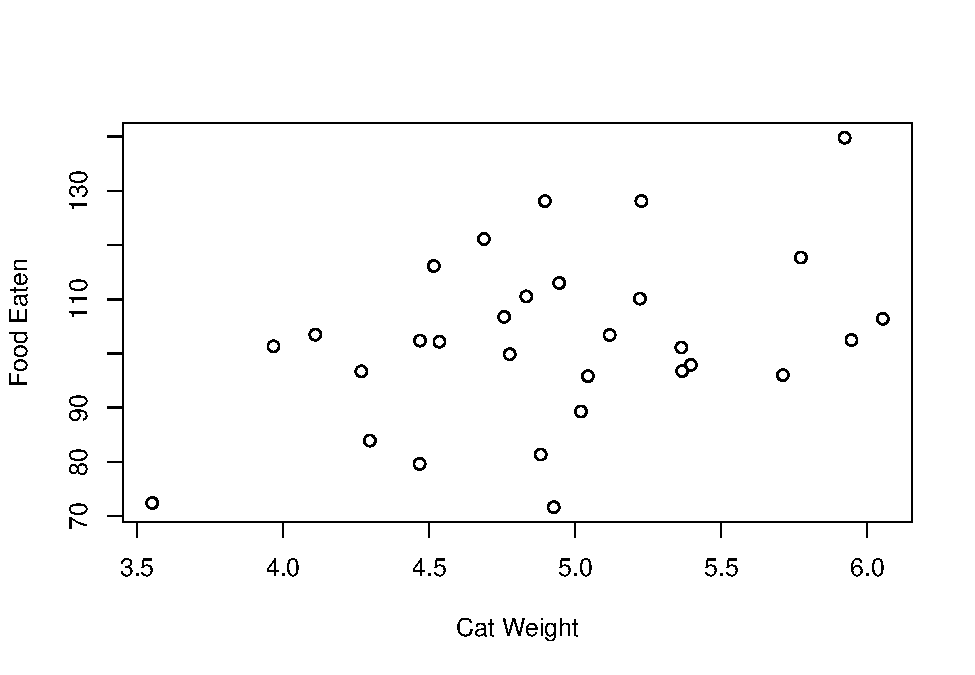
\includegraphics{Basics_of_Regression_files/figure-latex/unnamed-chunk-3-1.pdf}

\section{How can we describe these
data?}\label{how-can-we-describe-these-data}

\begin{itemize}
\tightlist
\item
  There is a lot of variability.
\item
  But the heavier cats do seem to eat a little bit more.
\item
  That's not a terribly precise statement
\item
  Can we use maths to make a better one?
\item
  Maybe we could draw a line through the points and then describe the
  line?
\end{itemize}

\section{Fitting a line to the data}\label{fitting-a-line-to-the-data}

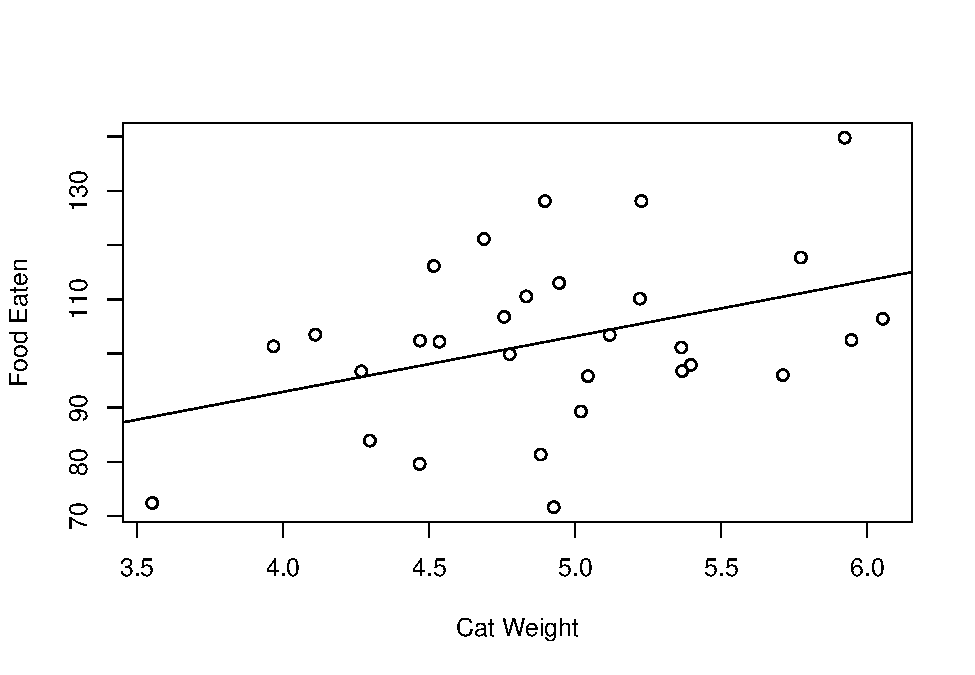
\includegraphics{Basics_of_Regression_files/figure-latex/unnamed-chunk-4-1.pdf}
- Looks like we have a strong positive relationship: The heavier the cat
(variable \(x\)), the more food eaten (variable \(y\)).

\section{Fitting a line to the data}\label{fitting-a-line-to-the-data-1}

\begin{itemize}
\tightlist
\item
  What is this line?
\item
  There are lots of possible lines to draw for data like these

  \begin{itemize}
  \tightlist
  \item
    What is the best line to describe these data?
  \item
    Remember (from school) that a line is (exhaustively) described by an
    equation such as \[y = a+b\cdot x\]
  \item
    \(a\) is called the \emph{intercept}. It describes where the line
    intersects the \(y\)-axis
  \item
    \(b\) is called the \emph{slope}. It describes by how many units
    \(y\) changes when \(x\) changes
  \item
    You may have learned this as \(y = mx + c\) depending on where you
    went to school
  \end{itemize}
\end{itemize}

\section{Errors}\label{errors}

\begin{itemize}
\tightlist
\item
  No line will ever fit the data perfectly (i.e.~go through all the
  points)
\item
  The difference between what the line \emph{predicts} for a certain Y
  value (the predition is called \(\hat{y}\)) and what the Y value
  actually is can be called the error \(E\):
\item
  For point i: \[E_i = Y_i - a + b\cdot X_i = Y_i - \hat{Y_i}\]
\end{itemize}

\section{\texorpdfstring{The ``best''
line?}{The best line?}}\label{the-best-line}

\begin{itemize}
\tightlist
\item
  How do we find the best \(a\) and \(b\) (i.e.~the best line) for the
  data?
\item
  Errors should sum to 0 (otherwise we are way off!)

  \begin{itemize}
  \tightlist
  \item
    This means the line should go through the point
    \((\bar{X}|\bar{Y})\)
  \end{itemize}
\item
  Smallest errors?
\item
  The errors are the difference between the values predicted by the line
  and the actual values:

  \begin{itemize}
  \tightlist
  \item
    We want the line that minimises all the deviations (in both
    directions) of the values predicted by the equation (\(\hat{Y}\))
    from the actual \(y\) values
  \end{itemize}
\end{itemize}

\section{Minimising the errors}\label{minimising-the-errors}

\begin{itemize}
\tightlist
\item
  Two possibilities here: We could just minimise the \emph{absolute
  value} of the deviations:
  \[\sum\limits_{i=1}^{n} \left|E_i\right| = \sum\limits_{i=1}^{n}\left|Y_i - \hat{Y}_i\right| =min\]

  \begin{itemize}
  \tightlist
  \item
    This is called \emph{least absolute values regression}, but it is
    quite mathematically complex, so it's rarely used and we won't talk
    about it in this unit.
  \item
    It's much easier to use squares instead of absolute values and
    perform a \emph{least squares regression}, so that is what almost
    everyone uses. Also, this puts a special penalty on large
    deviations, which is nice.
    \[\sum\limits_{i=1}^{n} E_i^2 = \sum\limits_{i=1}^{n}(Y_i - \hat{Y}_i)^2 =min\]
  \end{itemize}
\end{itemize}

\section{The least-Squares regression
line}\label{the-least-squares-regression-line}

\begin{itemize}
\tightlist
\item
  Here, I've plotted the errors, i.e.~the deviations of the predicted
  values (on the line) from the actual values. These are also called the
  \textbf{residuals}.
\end{itemize}

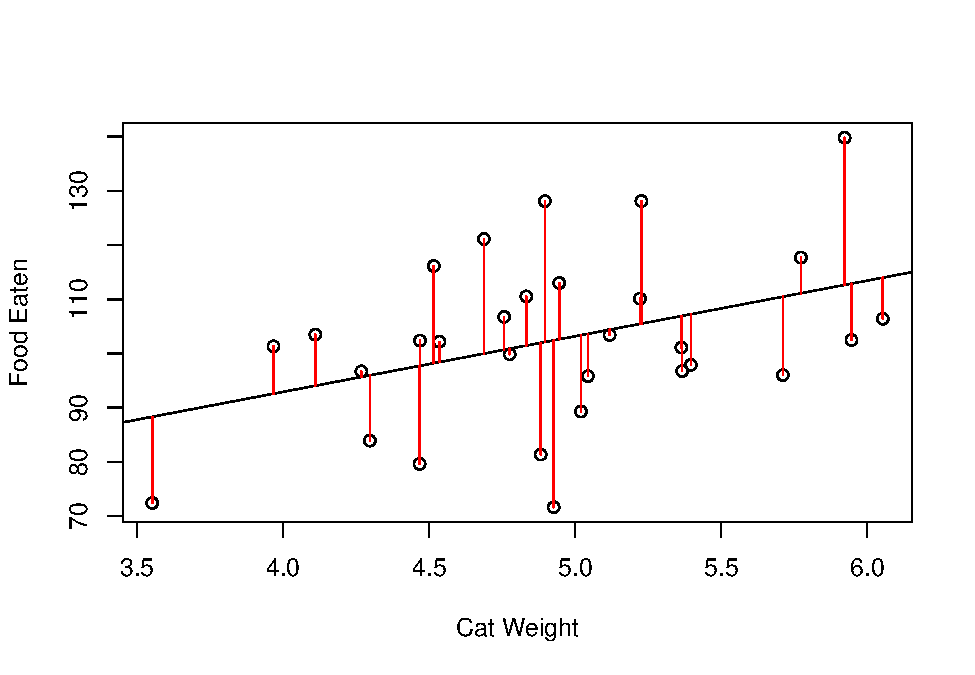
\includegraphics{Basics_of_Regression_files/figure-latex/unnamed-chunk-5-1.pdf}

\begin{itemize}
\tightlist
\item
  For the simple case where all we do is predict one \(y\) from one
  \(x\) variable, the \(b\) value is really easy to calculate. We start
  with the covariance.
\end{itemize}

\section{Covariance}\label{covariance}

\begin{itemize}
\tightlist
\item
  Defined as:
  \[cov(x, y) = \frac{\sum\limits_{i = 1}^n {(x_i - \bar{x})\cdot(y_i - \bar{y})}}{n-1}\]
\item
  The covariance gives us a measure of how much \(x\) and \(y\) vary
  together:

  \begin{itemize}
  \tightlist
  \item
    if \(x\)-values that are far away from the mean co-occur with \(y\)
    values that are also far from the mean, we get a large absolute
    covariance (it can be either positive or negative, depending on
    which way the relationship between \(x\) and \(y\) goes)
  \item
    if \(x\)-values that are far away from the mean co-occur with \(y\)
    values that are close to the mean (and vice-versa), we get a small
    absolute covariance (i.e. \(x\) and \(y\) don't change together)
  \end{itemize}
\end{itemize}

\section{Covariance, the regression slope, and
correlation}\label{covariance-the-regression-slope-and-correlation}

\begin{itemize}
\tightlist
\item
  Let's see if this is useful for our goal of getting a least-squares
  line:

  \begin{itemize}
  \tightlist
  \item
    We're still trying to minimise
    \(\sum\limits_{i=1}^{n} E_i^2 = \sum\limits_{i=1}^{n}(Y_i - A - B \cdot X_i )^2\)
  \item
    To minimise we'll have to use derivatives of this function. See the
    Fox (2013) book if you are truely interested.
  \end{itemize}
\end{itemize}

\section{Estimating the coefficients}\label{estimating-the-coefficients}

\begin{itemize}
\tightlist
\item
  In any case, it turns out that if we only have on independent
  (predictor) variable, we can compute the regression slope from the
  covariance: \[b = \frac{cov(x, y)}{s_x^2}\]
\item
  We can then get the intercept using the means of X and Y:
  \[a = \bar{Y} - b\cdot\bar{X}\]
\item
  That's it -- we have the function for our least squares regression
  line.
\end{itemize}

\section{Evaluating the linear model}\label{evaluating-the-linear-model}

\begin{itemize}
\tightlist
\item
  What we really want to know: How closely are the predictor variable
  and the predicted variable related?
\item
  Two ways to think about this.

  \begin{itemize}
  \tightlist
  \item
    First way: Think about the two coefficients in the linear model: the
    intercept \(a\) and the slope \(b\)
  \item
    Which one is indicative of the relationship between predictor and
    predicted variables?
  \item
    The slope of course!
  \end{itemize}
\end{itemize}

\section{Interpreting the slope}\label{interpreting-the-slope}

\begin{itemize}
\tightlist
\item
  Can we interpret \(b\) directly?

  \begin{itemize}
  \tightlist
  \item
    Clearly, the larger \(b\) is the better the prediction
  \item
    But \(b\) depends on the scales of predicted and predictor variables

    \begin{itemize}
    \tightlist
    \item
      Tricky to compare!
    \item
      Can we standardise somehow?
    \item
      Yes! We get the \textbf{correlation} \(r\) if we standardise the
      covariance by dividing it by the product of the standard
      deviations (\(s_x \cdot s_y\)). In short,
      \(r = \frac{cov(x, y)}{s_x \cdot s_y}\).
    \end{itemize}
  \end{itemize}
\end{itemize}

\section{Other approach: Sums of
squares}\label{other-approach-sums-of-squares}

\begin{itemize}
\tightlist
\item
  We can also express how well our model predicts the data as
  \textbf{sums of squares}
\item
  The total sums of squares is simply the numerator of the variance of
  \(y\): \({SS}_{total} = \sum\limits_{i=1}^{n}(y_i - \bar{y})^2\)
\item
  The \textbf{regression} or model sums of squares is the variance
  explained by the regression model:
  \({SS}_{model} = \sum\limits_{i=1}^{n}(\hat{y}_i - \bar{y})^2\)
\item
  The residual sums of squares is the squared differences \(e_i\)
  between the actual \(y\)-values and the predicted \(\hat{y}\)-values:
  \({SS}_{residual} = \sum\limits_{i=1}^{n}e_i = \sum\limits_{i=1}^{n}(y_i - \hat{y}_i)^2\)
\end{itemize}

\section{Coefficient of
determination}\label{coefficient-of-determination}

\begin{itemize}
\tightlist
\item
  How much of the variance of the data is determined (explained) by the
  model? \[r^2 = \frac{{SS}_{model}}{{SS}_{total}}\]
\item
  \(\frac{{SS}_{model}}{{SS}_{total}}\) is the same as the square of the
  correlation coefficient \(r\).

  \begin{itemize}
  \tightlist
  \item
    Fun activity at home: Work out why!
  \end{itemize}
\item
  In multiple regression, we call the coefficient of determination
  \(R^2\) instead of \(r^2\). Here, we have multiple predictors and
  multiple correlations, so \(R^2\) doesn't correspond to the square of
  any one of them. It still tells you how much variance your model
  explains, though.
\item
  In our example: \(r^2 = 0.154\)
\end{itemize}

\section{Statistical inference for
regression}\label{statistical-inference-for-regression}

\begin{itemize}
\tightlist
\item
  This lecture corresponds to Chapter 6 in Fox (2013)
\item
  You can find the more involved details (such as a lot of the
  derivations) there
\item
  Goals for this lecture:
\item
  Learn how to do hypothesis tests on least-squares regression results

  \begin{itemize}
  \tightlist
  \item
    For individual predictors (t-tests)
  \item
    For entire models (F-tests)
  \item
    Learn how to use SPSS to perform these tests for you
  \end{itemize}
\item
  Learn about assumptions that need to be true so you can perform these
  tests
\item
  Introduction to the problem of \textbf{multicollinearity}
\end{itemize}

\section{Hypothesis tests (for simple
regression)}\label{hypothesis-tests-for-simple-regression}

\begin{itemize}
\tightlist
\item
  When we do a regression analysis, we \emph{assume} that there is a
  true linear relationship in our population :
  \[Y_i = \alpha + \beta\cdot x_i + \varepsilon_i\]
\item
  \(\alpha\) and \(\beta\) are our population coefficients.
  \(\varepsilon_i\) is the error for this particular observation.
\end{itemize}

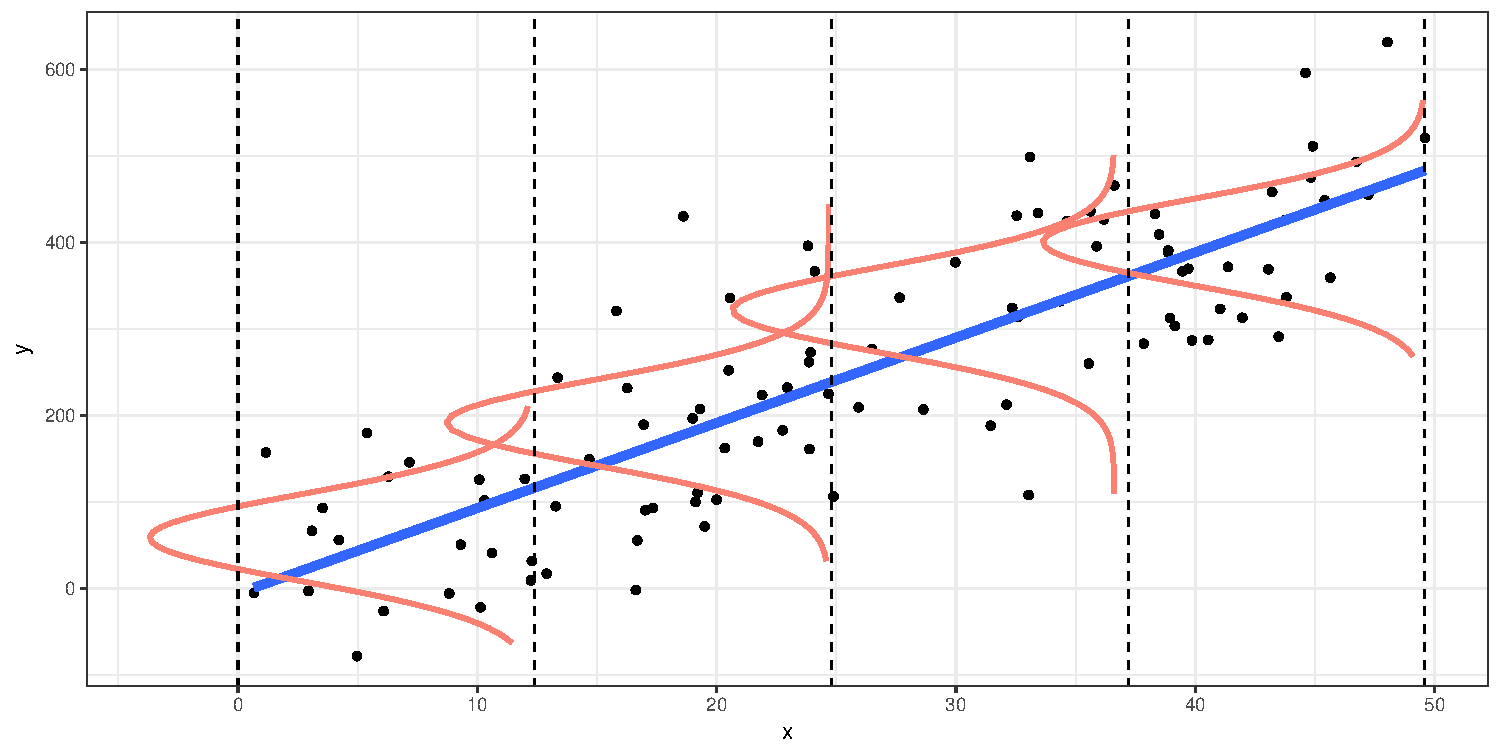
\includegraphics{Basics_of_Regression_files/figure-latex/unnamed-chunk-6-1.pdf}

\section{Hypothesis tests (for simple
regression)}\label{hypothesis-tests-for-simple-regression-1}

\begin{itemize}
\tightlist
\item
  We will need to estimate our regression equation based on our sample,
  so that \(a\) and \(b\) are estimates of the population coefficients
  \(\alpha\) and \(\beta\).
\item
  \(\varepsilon\) is the \textbf{error}. It represents all the
  influences (random or not) that we are not considering in the linear
  relationship.

  \begin{itemize}
  \tightlist
  \item
    If the relationship is actually linear, then \(E(\varepsilon) = 0\)
  \end{itemize}
\item
  How can we interpret these estimated coefficients? Mostly, we care
  about whether \(\beta = 0\) or not, i.e.~whether there is or isn't a
  significant relationship between \(x\) and \(y\) in the population.
\end{itemize}

\section{Assumptions}\label{assumptions}

\begin{itemize}
\tightlist
\item
  First, we need to assume that \(x\) and \(y\) come from a
  \textbf{bivariate} normal distribution (i.e.~that they are both
  normally distributed) with means \(\mu_x\) and \(\mu_y\), variances
  \(\sigma^2_x\) and \(\sigma^2_y\), and covariance \(\sigma_{x,y}\).
\item
  The bivariate (or, more generally, multivariate) normal distribution
  assumes that:

  \begin{itemize}
  \tightlist
  \item
    For each \(x\)-value \(x_j\), the corresponding
    \(y_{(i|x_j)}\)-values are normally distributed:
    \(\epsilon \sim N(0, \sigma_{\epsilon}^2\))
  \item
    For each \(x\)-value \(x_j\), the corresponding
    \(y_{(i|x_j)}\)-values have the same standard deviation
    (homoscedasticity assumption):
    \(Var(\epsilon_i) = \sigma_{\epsilon}^2\)
  \item
    For each \(x\)-value \(x_j\), the corresponding
    \(y_{(i|x_j)}\)-values are independent (i.e.~all \(\epsilon_i\) are
    independent)
  \end{itemize}
\end{itemize}

\section{Distribution of the coefficient estimates:
Means}\label{distribution-of-the-coefficient-estimates-means}

\begin{itemize}
\tightlist
\item
  If our assumptions are met, our coefficient estimates \(A\) and \(B\)
  will be themselves normally distributed
\item
  What do their distributions look like?

  \begin{itemize}
  \tightlist
  \item
    Expected values (i.e.~means): \(E(A) = \alpha\); \(E(B) = \beta\)

    \begin{itemize}
    \tightlist
    \item
      The coefficients are unbiased estimators of the population
      coefficients
    \end{itemize}
  \end{itemize}
\end{itemize}

\section{Distribution of the coefficient estimates:
Variances}\label{distribution-of-the-coefficient-estimates-variances}

\begin{itemize}
\tightlist
\item
  What about the variance?
\item
  We don't really care about \(Var(A)\) (see page 109 in Fox, 2015), but
  \(Var(B)\) is important for our hypothesis tests:
  \[Var(B) = \frac{\sigma_{\varepsilon}^2}{\sum\limits_{i=1}^{n}(x_i-\bar{x})^2} = \frac{\sigma_{\varepsilon}^2}{(n-1)\cdot s^2_{x}}\]
\item
  This means that the sampling variance of our estimate of \(\beta\)
  will be smaller when:

  \begin{itemize}
  \tightlist
  \item
    Numerator: the overall error variance \(\sigma_{\varepsilon}^2\) is
    small
  \item
    Denominator: we have a large number of observations \((n-1)\) and
    \(x\)-values in our sample are spread out (the sample variance of
    \(x\), \(S_x^2\) is larger)
  \end{itemize}
\end{itemize}

\section{Doing a hypothesis test on
B}\label{doing-a-hypothesis-test-on-b}

\begin{itemize}
\tightlist
\item
  We now know the sampling distribution of \(B\) (if our assumptions are
  met):
  \[ B \sim N\left(\beta, \frac{\sigma_{\varepsilon}^2}{\sum\limits_{i=1}^{n}(x_i-\bar{x})^2}\right)\]
\item
  But we don't know \(\sigma_{\varepsilon}^2\)

  \begin{itemize}
  \tightlist
  \item
    Does this remind you of something?
  \item
    Can we estimate this variance?
  \end{itemize}
\end{itemize}

\section{Doing a hypothesis test on B when the error variance is not
known}\label{doing-a-hypothesis-test-on-b-when-the-error-variance-is-not-known}

\begin{itemize}
\tightlist
\item
  (i.e.~pretty much in any situation)
\item
  Remember what we did in Lecture 3: we took the sample variance to
  estimate the population variance
\item
  Now we estimate the error in the population \(\sigma_\varepsilon^2\)
  by the error in the sample \(S^2_E\):
  \[S^2_E = \frac{\sum\limits_{i = 1}^{n} E_i^2}{n-2} = \frac{\sum\limits_{i = 1}^{n} (Y_i - \hat{Y}_i)^2}{n-2}\]

  \begin{itemize}
  \tightlist
  \item
    Why divide by \(n-2\)? So we get an unbiased estimator of the error.
    Not showing you the derivation of why it has to be \(n-2\).
  \end{itemize}
\item
  Remember this? We are \emph{estimating} both the mean and the error
  variance from the sample, so we need to use the \emph{t}-distribution
  instead of the standard normal distribution.
\end{itemize}

\section{Testing coefficients}\label{testing-coefficients}

\begin{itemize}
\tightlist
\item
  Our null hypothesis is usually \(H_0: \beta = 0\)

  \begin{itemize}
  \tightlist
  \item
    i.e.~there is no systematic relationship between \(x\) and \(y\);
    you can't predict \(y\) from \(x\)
  \end{itemize}
\item
  We already have our best estimate of \(\beta\) (the coefficient \(B\)
  calculated from the sample). We still need an estimate for the
  standard error of \(B\). We take the definition of \(Var(B)\) from
  above and plug in \(S_E^2\) for \(\sigma_{\varepsilon}^2\)
  \[SE(B) = \sqrt{Var(B)} = \sqrt{\frac{S^2_E}{\sum\limits_{i=1}^{n}(x_i-\bar{x})^2}}= \frac{S_E}{\sqrt{\sum\limits_{i=1}^{n}(x_i-\bar{x})^2}}\]
\end{itemize}

\section{Calculating the t-value}\label{calculating-the-t-value}

\begin{itemize}
\tightlist
\item
  We calculate a \emph{t}-value for our observed slope coefficient \(B\)
  just like we do when we're comparing means
  \[t = \frac{B - \beta_0}{SE(B)}\] where \(\beta_0\) is the value of
  \(\beta\) assumed by the null hypothesis.

  \begin{itemize}
  \tightlist
  \item
    Usually, \(\beta_0 = 0\), so we can rewrite this as
    \(t = \frac{B}{SE(B)}\)
  \end{itemize}
\item
  As always, this \emph{t}-value has as many degrees of freedom as the
  denominator of the estimated variance. In the case of the error
  variance, \(df_t = n-2\).
\item
  We can also get confidence intervals, just like when comparing means:
  \(CI: B \pm t_{\alpha/2}\cdot SE(B)\). We reject the \(H_0\) if the CI
  doesn't include 0.
\end{itemize}

\section{Back to our example from last
week}\label{back-to-our-example-from-last-week}

\begin{itemize}
\tightlist
\item
  Remember, we're trying to predict cat food eaten from cat weight.
\end{itemize}

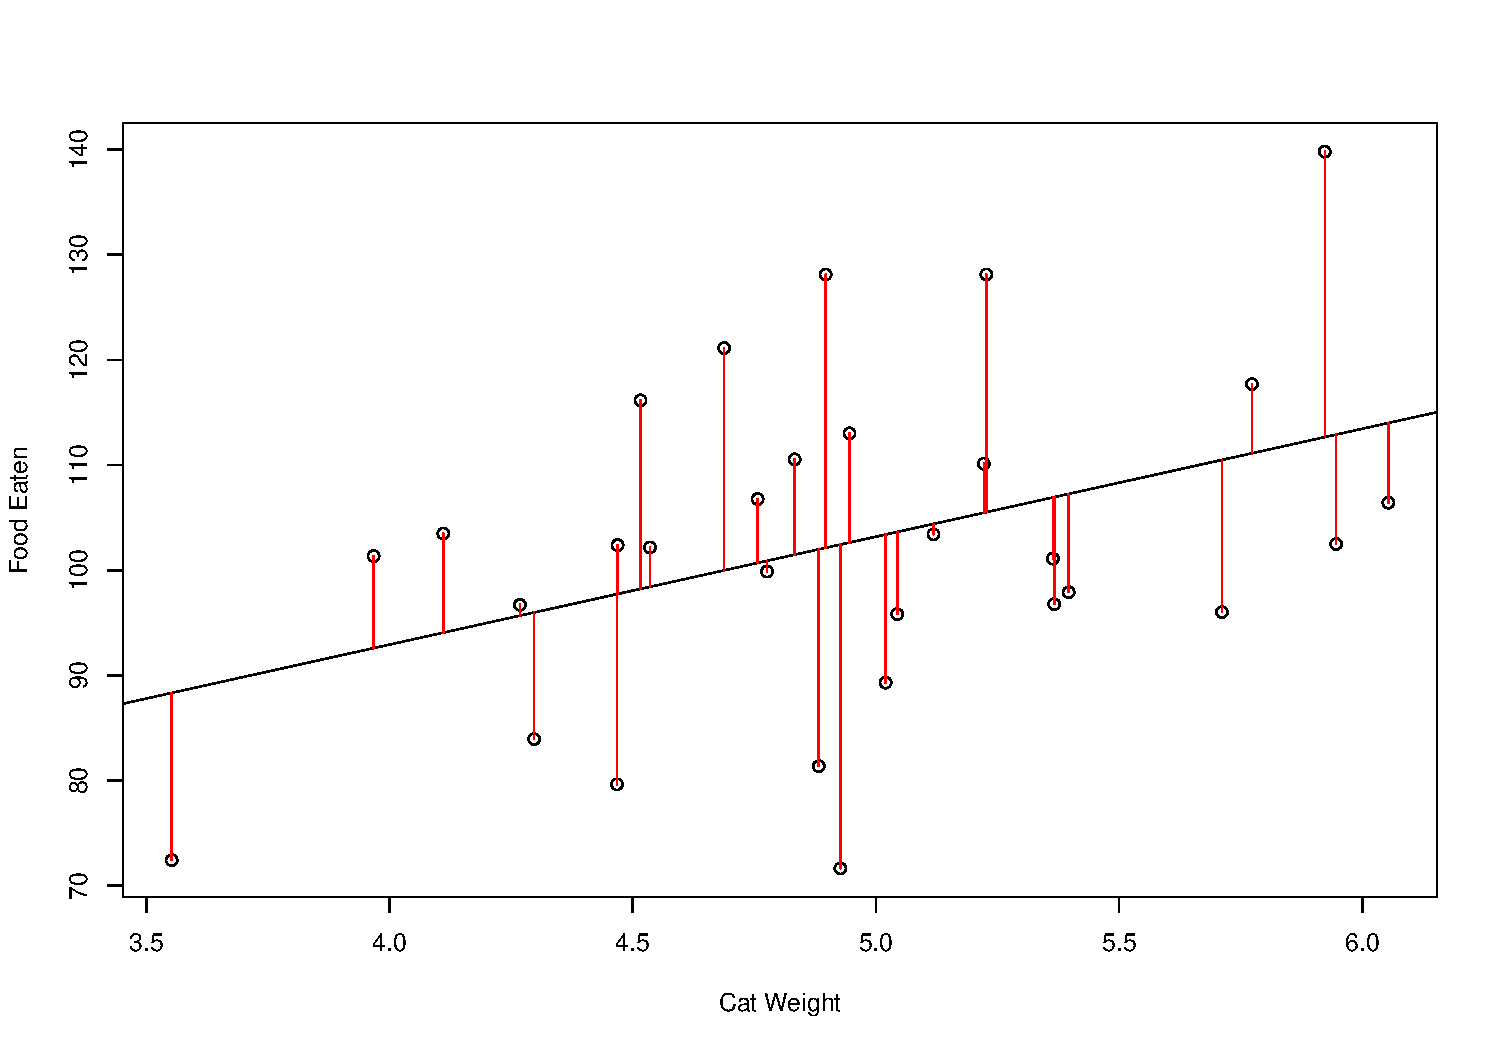
\includegraphics{Basics_of_Regression_files/figure-latex/unnamed-chunk-7-1.pdf}

\section{Calculating the
coefficients}\label{calculating-the-coefficients}

\begin{itemize}
\item
  We can calculate \(B\) from the data by first getting the covariance:
  \[
  \begin{aligned}
  &Cov(CatWeight,FoodEaten) \\ &= \frac{\sum\limits_{i = 1}^n {(CatWeight_i - \overline{CatWeight})\cdot(FoodEaten_i - \overline{FoodEaten})}}{n-1} \\ &= 3.766
  \end{aligned}\]
\item
  Then
  \[B = \frac{Cov(CatWeight, CatFood)}{S_{CatWeight}^2} = \frac{3.766}{0.367} = 10.261\]
\end{itemize}

\section{Calculating the t-value}\label{calculating-the-t-value-1}

\begin{itemize}
\tightlist
\item
  Now calculate the standard error of \(B\) (replacing \(CatWeight\)
  with \(x\) and \(CatFood\) with \(Y\) for better readability):
  \[SE(B) = \frac{S_E^2}{(n-1)\cdot S^2_{x}} = \frac{\frac{\sum\limits_{i = 1}^{n} (Y_i - \hat{Y}_i)^2}{n-2}}{(n-1)\cdot S^2_{x}} = \frac{\frac{6146.544}{30 - 2}}{(30 - 1)\cdot 0.367} = 20.626\]
\item
  And the \(t\)-value:
  \[t_{28} = \frac{B}{SE(B)} = \frac{10.261}{\sqrt{20.626}} = \frac{10.261}{4.542} = 2.259\]
\item
  The degrees of freedom are \(n-2=28\) (number of observations minus 1
  for the intercept and 1 for the slope).
\end{itemize}

\section{p-value and significance
test}\label{p-value-and-significance-test}

\begin{itemize}
\tightlist
\item
  Finally, look up the \emph{p}-value (e.g.~in Excel):
  \(p(|t_{28}| = 2.259) = 0.016\)
\item
  Remember, we are doing a two-tailed test, so we have to multiply the
  p-value by 2 if we want to compare it to \(\alpha = .05\):
  \(p =0.032\)
\item
  Looks like we can reject the \(H_0\) this time: Heavier cats tend to
  eat more.
\end{itemize}

\section{Alternative: Do an F-Test to compare
variances}\label{alternative-do-an-f-test-to-compare-variances}

\begin{itemize}
\tightlist
\item
  Remember, an F-Value is is what you get when you divide a chi-square
  value by another chi-square value

  \begin{itemize}
  \tightlist
  \item
    That is, when you divide one variance estimate by another
  \end{itemize}
\item
  Basically, we compare the variance explained by the model with the
  error variance

  \begin{itemize}
  \tightlist
  \item
    If there is no effect, the variance attributed to the model will be
    solely due to random error, as will be the error variance (of
    course).
  \item
    So, if there is no effect, the expected values of both variance
    estimates should be the same, and if you divide one by the other you
    should get an F-value close to 1.
  \item
    You can occasionally get an F-value greater than one. The
    F-distribution tells you how likely that is given that the null
    hypothesis is true.
  \end{itemize}
\end{itemize}

\section{Calculating the F-value}\label{calculating-the-f-value}

\begin{itemize}
\tightlist
\item
  Let's calculate the variance estimates. First the variance explained
  by the model.

  \begin{itemize}
  \tightlist
  \item
    We start with sums of squares (SS)

    \begin{itemize}
    \tightlist
    \item
      \(SS_{model}\): The variance explained by the regression model.
      The sum of squared differences between the predicted values and
      the mean.
      \[SS_{model} = \sum\limits_{i=1}^{n}(\hat{Y}_i - \bar{Y})^2\]
    \item
      \(SS_{error}\): The variance that isn't explained by the
      regression model, i.e.~the residual or error variance. The sum of
      squared differences between the actual values and the predicted
      values. \[SS_{error} = \sum\limits_{i=1}^{n}(Y_i - \hat{Y}_i)^2\]
    \end{itemize}
  \end{itemize}
\end{itemize}

\section{Relationship between the sums of
squares}\label{relationship-between-the-sums-of-squares}

\begin{itemize}
\tightlist
\item
  We partition the total variance between model and error variance\\
\item
  \(SS_{total}\): The overall variance. The sum of squared differences
  between the actual values and the mean.
  \[SS_{total} = \sum\limits_{i=1}^{n}(y_i - \bar{y}_i)^2\]
\item
  \(SS_{model}\) and \(SS_{error}\) sum up to \(SS_{total}\):
  \[SS_{total} = SS_{model} + SS_{error}\]
\end{itemize}

\section{Degrees of freedom}\label{degrees-of-freedom}

\begin{itemize}
\tightlist
\item
  In order to actually get variance estimates, we have to divide the SS
  by their degrees of freedom.
\item
  \(df_{model} = p - 1\), where p is the number of regression parameters
  (intercept and slopes)
\item
  \(df_{error} = n - p\), where \(n\) is the number of observations and
  \(p\) is the number of regression parameters.
\item
  \(df_{total} = n - 1\), where \(n\) is the number of observations
\item
  \(df_{model} + df_{error} = df_{total}\)
\end{itemize}

\section{Mean squares}\label{mean-squares}

\begin{itemize}
\tightlist
\item
  In order to get variance estimates, we have to divide the sums of
  squares by their degrees of freedom
\item
  For the cat example:
  \(MS_{model} = \frac{SS_{model}}{df_{model}} = \frac{\sum\limits_{i=1}^{n}(\hat{Y}_i - \bar{Y})^2}{1} = 1120.577\)
\item
  \(MS_{error} = \frac{SS_{error}}{df_{error}} = \frac{\sum\limits_{i=1}^{n}E_i = \sum\limits_{i=1}^{n}(Y_i - \hat{Y}_i)^2}{n-2} = \frac{6146.544}{30 - 2} = 219.519\)
\end{itemize}

\section{F-test}\label{f-test}

\begin{itemize}
\tightlist
\item
  \(F_{(1, 28)} = \frac{MS_{model}}{MS_{residual}} = \frac{1120.577}{202.885} = 5.105\)
\item
  \(p(F_{(1, 28)} = 5.105) = 0.032\)
\item
  Guess what? The square root of the \emph{F}-value is our
  \emph{t}-value. This only works if we have one single predictor:
  \(\sqrt{F_{(1,28)}} = t_{28} = 2.259\)
\end{itemize}

\section{Summary: What did we find?}\label{summary-what-did-we-find}

\begin{itemize}
\tightlist
\item
  The best fitting line for the cat food data intersects the \(y\)-axis
  at the point (0, 51.885).
\item
  (We never bothered to estimate \(a\) by hand, but that's what you
  would get.)
\item
  Not all x-values are sensible for all data. Saying that a cat with 0
  kg weight would eat 51.885 g of food makes no sense, since a cat with
  0 kg weight is not a cat.
\item
  The linear function doesn't care, of course. It knows nothing about
  our data and just specifies a line.
\item
  The slope might be more useful: It says that for each kg of extra
  weight, a cat will eat 10.261 more grammes of food.

  \begin{itemize}
  \tightlist
  \item
    Using this information, we can predict that a giant 8 kg cat would
    eat \(51.885 + 10.261 \cdot 8 = 133.973\) g of food.
  \end{itemize}
\end{itemize}

\section{Summary: Predictions and residual
errors}\label{summary-predictions-and-residual-errors}

\begin{itemize}
\tightlist
\item
  Of course, our prediction is likely to be at least a little off.
\item
  If we had an 8 kg cat in our data and its actual amount of food
  consumed was 170 g, we'd have an error of \(E_i = 36.027\).
\item
  This is called the residual error.
\item
  More formally, the \textbf{population} regression equation looks like
  this (where \(x_i\) are the individual values for the \(x\) variable,
  and \(y_i\) are the corresponding values for the \(Y\) variable):

  \begin{itemize}
  \tightlist
  \item
    \(y_i = \alpha + \beta_1 x_i + \varepsilon_i\)
  \item
    Here, we've simply renamed the intercept to \(\alpha\) and the slope
    to \(\beta_1\).
  \item
    \(\varepsilon_i\) is the residual error for each data point.
  \item
    Important: \(\varepsilon_i\) is assumed to be normally distributed
  \item
    This doesn't matter for the line fitting, but it does for the
    hypothesis tests!
  \end{itemize}
\end{itemize}

\section{Summary: Hypothesis testing}\label{summary-hypothesis-testing}

\begin{itemize}
\tightlist
\item
  Important: Note that the \(\beta\) variables are greek letters, which
  means they are the \emph{population parameters}
\item
  For each \(\beta\) coefficient in the regression formula, we can
  propose the \(H_0\) that the true value of that \(\beta\) coefficient
  is 0
\item
  The \(\beta\) that are estimated from our sample are simply called
  \(B\)
\item
  We can once again test if our \(B\) values are extreme enough so they
  would only occur 5\% of the time or less given the \(H_0\).
\item
  We test this separately for each \(B\) value. Guess what, it's a
  \emph{t}-test (an F-test is also possible)!
\item
  We can also test whether the intercept \(A\) is 0

  \begin{itemize}
  \tightlist
  \item
    This is usually not particularly interesting unless you have a very
    specific hypothesis about the intercept.
  \end{itemize}
\end{itemize}

\section{Multiple regression}\label{multiple-regression}

\begin{itemize}
\tightlist
\item
  Unlike simply running a hypothesis test on a correlation, we can
  easily add another predictor to a linear model, making it a multiple
  regression model, where \(x_{1i}\) is observation \emph{i} on the
  first predictor and \(x_{2i}\) is observation \emph{i} on the second
  predictor:

  \begin{itemize}
  \tightlist
  \item
    \(Y_i = \alpha + \beta_1 x_{1i} + \beta_2 x_{2i} + \beta_3 x_{1,i} \cdot x_{2,i} + \varepsilon_i\)
  \item
    Note that we have an interaction term in this equation:
    \(\beta_3 x_{1,i} \cdot x_{2,i}\)
  \item
    We could also specify the model without the interaction if we think
    there might be a possibility that the effects are just additive:

    \begin{itemize}
    \tightlist
    \item
      \(y_i = \alpha + \beta_1 x_{1i} + \beta_2 x_{2i} + \varepsilon_i\)
    \end{itemize}
  \item
    Which of the models is better?
  \item
    That's exactly what we want to find out!
  \end{itemize}
\end{itemize}

\section{Hypothesis testing in multiple
regression}\label{hypothesis-testing-in-multiple-regression}

\begin{itemize}
\tightlist
\item
  Getting the least-squares coefficients \(A\) and \(B_1\), \(B_2\),
  etc. from the sample is computationally intensive in multiple
  regression. Let's leave this to Excel/SPSS.
\item
  Once we have the coefficients, we would of course like to run
  hypothesis tests on them (mostly the slopes).
\item
  If the assumptions (see above) are true, then the sample coefficients
  are unbiased estimators of the population coefficients. So \(B_1\)
  will be distributed around \(\beta_1\) and so on.
\item
  But what is the sampling variance of the estimates?

  \begin{itemize}
  \tightlist
  \item
    We can estimate the error variance from the sample again:
    \(S_E^2 = \frac{\sum E_i^2}{n-k-1}\), where \(n\) is the number of
    observations and \(k\) is the number of predictors.
  \end{itemize}
\end{itemize}

\section{The sampling variance of each
B}\label{the-sampling-variance-of-each-b}

\begin{itemize}
\tightlist
\item
  Each predictor \(X_j\) has its own coefficient \(B_j\) (i.e. \(X_1\)
  has \(B_1\) and so on as seen above)
\item
  The sampling variance is different for each \(B_j\) (i.e. \(B_1\),
  \(B_2\), \(B_3\), and so on)
  \[ Var(B_j) = \frac{1}{1-R_j^2} \cdot \frac{\sigma_\varepsilon^2}{\sum\limits_{i=1}^{n}(x_{ij}-\bar{x_j})^2}\]
\item
  Let's take this apart:
\item
  \(\frac{\sigma_\varepsilon^2}{\sum\limits_{i=1}^{n}(x_{ij}-\bar{x_j})^2}\)
  is what we already know from single regression: the error variance
  over the variability in \(x_j\)
\item
  The first part, \(\frac{1}{1-R_j^2}\) is new. It is called the
  Variance Inflation Factor (VIF).
\end{itemize}

\section{Variance Inflation Factor
(VIF)}\label{variance-inflation-factor-vif}

\begin{itemize}
\tightlist
\item
  The greater the VIF, the greater the variance and standard error of
  \(B_j\). In other words, the greater the VIF, the greater the
  uncertainty about the estimate of \(\beta_j\).

  \begin{itemize}
  \tightlist
  \item
    Remember that we divide by \(SE(B)\) to get the t-value. The greater
    the SE of \(B_j\), the lower the t-value will be. The lower the
    t-value, the higher the p-value.
  \end{itemize}
\item
  So, what influences the VIF? \(\frac{1}{1-R_j^2}\)
\item
  \(R_j^2\) is the squared multiple correlation coefficient between
  \(X_j\) and all the other predictors (the other \(X\) s).
\item
  The higher \(R_j^2\), the higher the VIF.

  \begin{itemize}
  \tightlist
  \item
    The closer \(X_j\) is related to the other predictors, the worse is
    our estimate \(B_j\). This is called the effect of
    \textbf{multicollinearity}.
  \end{itemize}
\end{itemize}

\section{Finishing the hypothesis
test}\label{finishing-the-hypothesis-test}

\begin{itemize}
\tightlist
\item
  Once we have \(Var(B)\) and \(SE(B) = \sqrt{Var(B)}\), we can
  calculate t-values for the coefficients as above. Each t-value tests
  the hypothesis \(H_0^{(k)}: \beta_k = 0\)
\item
  The degrees of freedom of the t-values are, once again, the
  denominator of \(S_E^2\) (see above): \(n-k-1\), where \(n\) is the
  number of observations and \(k\) is the number of predictors
\item
  You can also run an F-test. Partitioning the sums of squares works
  just like in the simple variance example.
\item
  \(df_{model}\) is the number of predictors \(k\), and \(df_{error}\)
  is \(n-k-1\).
\item
  This tests the \emph{omnibus} hypothesis that all slopes are 0:
  \(H_0: \beta_1 = \beta_2 = \dots = \beta_k = 0\).
\item
  This is not the same as testing the individual hypotheses (as we will
  see!)
\item
  You can also compare the \(SS_{model}\) of two different models.
\end{itemize}

\section{Example}\label{example-1}

\begin{itemize}
\tightlist
\item
  Let's assume that, apart from each cat's weight in kg, we also have
  its age in months:
\end{itemize}

\begin{longtable}[]{@{}rrr@{}}
\toprule
CatWeight & CatAge & FoodEaten\tabularnewline
\midrule
\endhead
5.37 & 25.84 & 96.8\tabularnewline
5.40 & 18.77 & 97.9\tabularnewline
4.27 & 62.42 & 96.7\tabularnewline
5.95 & 30.85 & 102.5\tabularnewline
4.47 & 21.75 & 79.6\tabularnewline
4.93 & 9.02 & 71.6\tabularnewline
\bottomrule
\end{longtable}

\begin{itemize}
\tightlist
\item
  Does adding age to the model improve it?
\item
  This will be our first adventure in SPSS. Feel free to follow along.
  The data file is in the lecture module on myBU.
\item
  Let's open the file \texttt{catfood\_age.csv} from myBU in SPSS
\end{itemize}

\section{The regression output}\label{the-regression-output}

\begin{itemize}
\tightlist
\item
  Calculating the coefficients in multiple regression gets
  computationally intense, so let's leave this to SPSS
\item
  First, let's fit the model without the interaction.
\item
  The output below is not from SPSS, but very similar:
\end{itemize}

\begin{verbatim}
## 
## Call:
## lm(formula = FoodEaten ~ CatWeight + CatAge, data = catfood_age)
## 
## Residuals:
##    Min     1Q Median     3Q    Max 
## -20.81  -5.41   1.49   4.46  27.94 
## 
## Coefficients:
##             Estimate Std. Error t value Pr(>|t|)    
## (Intercept) -10.4377    19.7290   -0.53      0.6    
## CatWeight    17.7645     3.5024    5.07 0.000025 ***
## CatAge        0.4555     0.0847    5.38 0.000011 ***
## ---
## Signif. codes:  0 '***' 0.001 '**' 0.01 '*' 0.05 '.' 0.1 ' ' 1
## 
## Residual standard error: 10.5 on 27 degrees of freedom
## Multiple R-squared:  0.592,  Adjusted R-squared:  0.562 
## F-statistic: 19.6 on 2 and 27 DF,  p-value: 0.00000557
\end{verbatim}

\section{Interpreting the
coefficients}\label{interpreting-the-coefficients}

\begin{itemize}
\item
  Let's look at just the coefficients:

  \begin{longtable}[]{@{}rllll@{}}
  \toprule
  Est & imate Std & . Error t v & alue Pr( &
  \textgreater{}\textbar{}t\textbar{})\tabularnewline
  \midrule
  \endhead
  (Intercept) & -10.438 & 19.729 & -0.529 & 0.601\tabularnewline
  CatWeight & 17.765 & 3.502 & 5.072 & 0.000\tabularnewline
  CatAge & 0.456 & 0.085 & 5.381 & 0.000\tabularnewline
  \bottomrule
  \end{longtable}
\item
  Looks like both the coefficient for CatWeight and the coefficient for
  CatAge are significantly different from 0
\end{itemize}

\section{Now let's add the interaction
term}\label{now-lets-add-the-interaction-term}

\begin{itemize}
\item
  Note that SPSS is a bit annoying about this, making you calculate the
  interaction term yourself

  \begin{longtable}[]{@{}rllll@{}}
  \toprule
  Est & imate Std & . Error t v & alue Pr( &
  \textgreater{}\textbar{}t\textbar{})\tabularnewline
  \midrule
  \endhead
  (Intercept) & 22.568 & 46.302 & 0.487 & 0.630\tabularnewline
  CatWeight & 11.357 & 8.853 & 1.283 & 0.211\tabularnewline
  CatAge & -0.067 & 0.668 & -0.101 & 0.920\tabularnewline
  CatWeight:CatAge & 0.103 & 0.131 & 0.789 & 0.437\tabularnewline
  \bottomrule
  \end{longtable}
\item
  Now nothing is significant! What is going on?
\item
  Important: these \emph{t}-tests test the null hypothesis that each
  individual coefficient is 0 \textbf{given that all the other
  predictors are in the model as well}.
\end{itemize}

\section{Our problem}\label{our-problem}

\begin{itemize}
\tightlist
\item
  This model is really hard to interpret

  \begin{itemize}
  \tightlist
  \item
    CatWeight or CatAge would have a strong effect individually
  \item
    But neither predictor adds anything if the interaction is already in
    the model
  \item
    Why? Because the interaction is strongly correlated with both of
    them!
  \end{itemize}
\item
  Make sure to check for correlations between predictors before running
  a regression

  \begin{itemize}
  \tightlist
  \item
    \texttt{Part-\ and\ partial\ correlations} in the
    \texttt{Statistics...} menu of the Linear Regression module
  \end{itemize}
\item
  Important: Some multicollinearity is unavoidable, but the more
  strongly your predictors are correlated, the more problems you get
\end{itemize}

\section{Diagnosing
Multicollinearity}\label{diagnosing-multicollinearity}

\begin{itemize}
\tightlist
\item
  SPSS actually gives you the VIF for each predictor
\item
  Click on ``Statistics\ldots{}'' and check ``Collinearity diagnostics''
\item
  They are in the coefficients table
\item
  For your convenience, the VIFs for this model are printed below
\end{itemize}

\begin{verbatim}
##        CatWeight           CatAge CatWeight:CatAge 
##             7.49            72.98            62.16
\end{verbatim}

\section{Interpreting the VIF}\label{interpreting-the-vif}

\begin{itemize}
\tightlist
\item
  You have a problem with multicollinearity if

  \begin{itemize}
  \tightlist
  \item
    The largest VIF is greater than 10 and/or
  \item
    The average VIF is substantially greater than 1
  \end{itemize}
\item
  Multicollinearity seriously affects the interpretability of your model
\item
  In practice, it increases the estimate of the standard error of your
  coefficients \(\sigma_{\beta}\)
\item
  This reduces the power of the significance test
\end{itemize}

\section{Where does the multicollinearity come
from?}\label{where-does-the-multicollinearity-come-from}

\begin{itemize}
\tightlist
\item
  Here's the problem: The interaction effect is equivalent to
  \(CatWeight \cdot CatAge\)
\item
  What to do? Luckily, there is an easy solution to this particular
  issue:
\item
  If we \textbf{center} both variables (i.e.~subtract the mean from each
  observation), the correlation will disappear
\item
  You can center variables using \texttt{Transform} --\textgreater{}
  \texttt{Compute\ Variable...}
\item
  Get the \textbf{mean} using \texttt{Analyze} --\textgreater{}
  \texttt{Descriptives...}, then subtract it from each observation of
  both variables:

  \begin{itemize}
  \tightlist
  \item
    \(CatWeight - 4.935\); \(CatAge - 55.52\)
  \end{itemize}
\item
  Save the new variables as \texttt{CatWeight\_centered} and
  \texttt{CatAge\_centered}
\end{itemize}

\section{Does this help?}\label{does-this-help}

\begin{longtable}[]{@{}lrrrr@{}}
\toprule
& Estimate & Std. Error & t value &
Pr(\textgreater{}\textbar{}t\textbar{})\tabularnewline
\midrule
\endhead
(Intercept) & 103.128 & 2.073 & 49.751 & 0.000\tabularnewline
Cat Weight & 17.082 & 3.632 & 4.704 & 0.000\tabularnewline
Cat Age & 0.441 & 0.087 & 5.069 & 0.000\tabularnewline
Cat Weight by Cat Age & 0.103 & 0.131 & 0.789 & 0.437\tabularnewline
\bottomrule
\end{longtable}

\begin{longtable}[]{@{}lr@{}}
\toprule
& VIF\tabularnewline
\midrule
\endhead
Cat Weight & 1.26\tabularnewline
Cat Age & 1.24\tabularnewline
Cat Weight by Cat Age & 1.07\tabularnewline
\bottomrule
\end{longtable}

\begin{itemize}
\tightlist
\item
  Yes, it does
\end{itemize}

\section{Let's look at the coefficients
again}\label{lets-look-at-the-coefficients-again}

\begin{table}[H]
\centering
\resizebox{\linewidth}{!}{\begin{tabular}{lrrrr}
\toprule
  & Estimate & Std. Error & t value & Pr(>|t|)\\
\midrule
(Intercept) & 103.128 & 2.073 & 49.751 & 0.000\\
CatWeight\_centered & 17.082 & 3.632 & 4.704 & 0.000\\
CatAge\_centered & 0.441 & 0.087 & 5.069 & 0.000\\
CatWeight\_centered:CatAge\_centered & 0.103 & 0.131 & 0.789 & 0.437\\
\bottomrule
\end{tabular}}
\end{table}

\begin{itemize}
\tightlist
\item
  Look at that: Now CatAge is significant, too!
\item
  We would have made a Type II error if we hadn't centered the
  variables.
\item
  Lesson of this story: When testing for interactions with continuous
  variables, \textbf{always center the continuous variables}.
\end{itemize}

\section{Why you always need to look at your
data}\label{why-you-always-need-to-look-at-your-data}

\begin{itemize}
\tightlist
\item
  These datasets all have the same regression line, but they look very
  different:
\end{itemize}

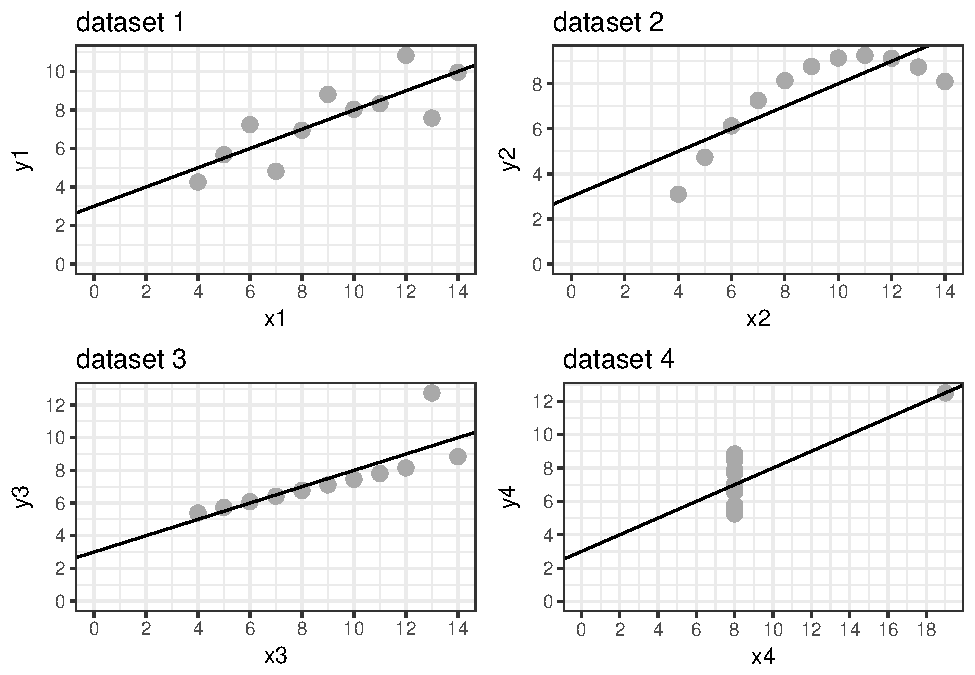
\includegraphics{Basics_of_Regression_files/figure-latex/unnamed-chunk-15-1.pdf}


\end{document}
